\chapter{Zer da HTML5?}

HTML5 zer den ulertzeko, lehenengo HTML zer den gogoratu behar dugu. HTML HyperText Markup Language edo Hiper Testua Markatzeko Lengoaia da. Webeko edukiek izan behar duten formatua definitzen duen estandarra, hain zuzen ere. Sir Tim Berners-Leek (webaren asmatzaileak) sortua 1991n, gaur egun
W3C (World Wide Web Consortium) erakundeak mantentzen du. HTML estandar internazionala bilakatu zen 2000n (ISO/IEC 15445:2000).

HTML lengoaia, CSS (Kaskadako Estilo Orriak edo Cascading Style Sheets) eta JavaScript lengoaia edozein webgune osatzeko erabiltzen diren oinarrizko teknologiak dira.

Web arakatzaileek (edo nabigatzaileek) HTML dokumentuak web zerbitzaritik edo disko gogorretik irakurri, interpretatu eta pantailan bistaratzen dituzte, testua, irudiak, bideoa eta audioa uztartuz.

HTML lengoaiaren historia interesgarria da, baina erakunde eta teknizismo asko uztartzen dituenez, beheko azpiatalean sartu dugu, hautazko irakurketa gisa. Datu bakar batekin geratuko gara: 2014a izan zen HTML5en lehenengo bertsio estandarra argitaratu zuten urtea.

Ez gara luzatuko HTML lengoiaren aurreko bertsioen (HTML4 eta aurrekoen) etiketak zehazten. Liburu hau irakurtzen ari bazara, ziur asko \textit{<h1>, <h2>, <p>, <font>, <i>, <a>, <img>, <form>, <input>, <textarea>} eta horrelakoak primeran menderatuko dituzu. 

Gaur egungo webguneak, berriz, ez dira lehengoak bezain errazak. Izan ere, gaur egungo web aplikazioak konplexuak, multimediadunak, mugikorrak eta \mbox{\textit{offline}} lan egin ahal izateko diseinatzen dira. Hori guztia lortzeko, ez dute inolako plugin edo gehigarririk erabiltzen (ez \textit{Flash}, ez \textit{JavaFX}, ez \textit{Silverlight}, ezer ere ez). HTML5, JavaScript eta CSS, besterik ez. Nola demontre lortu dute horrelako web aplikazioak egitea hiru osagai horiekin? HTML5 hitza da gakoa, eta ez bakarrik etiketa-lengoaia...

HTML5 etiketa-lengoaia, JavaScript-ek eskaintzen dituen zenbait API berri eta CSS3 lengoaia kutxa bakar batean sartzen baditugu, HTML5 etiketaz bataiatutako kutxa lortuko dugu. Ikusten denez, izen bakar batek zenbait kontzeptu izendatzen ditu.

\begin{figure}[ht]
	\centering
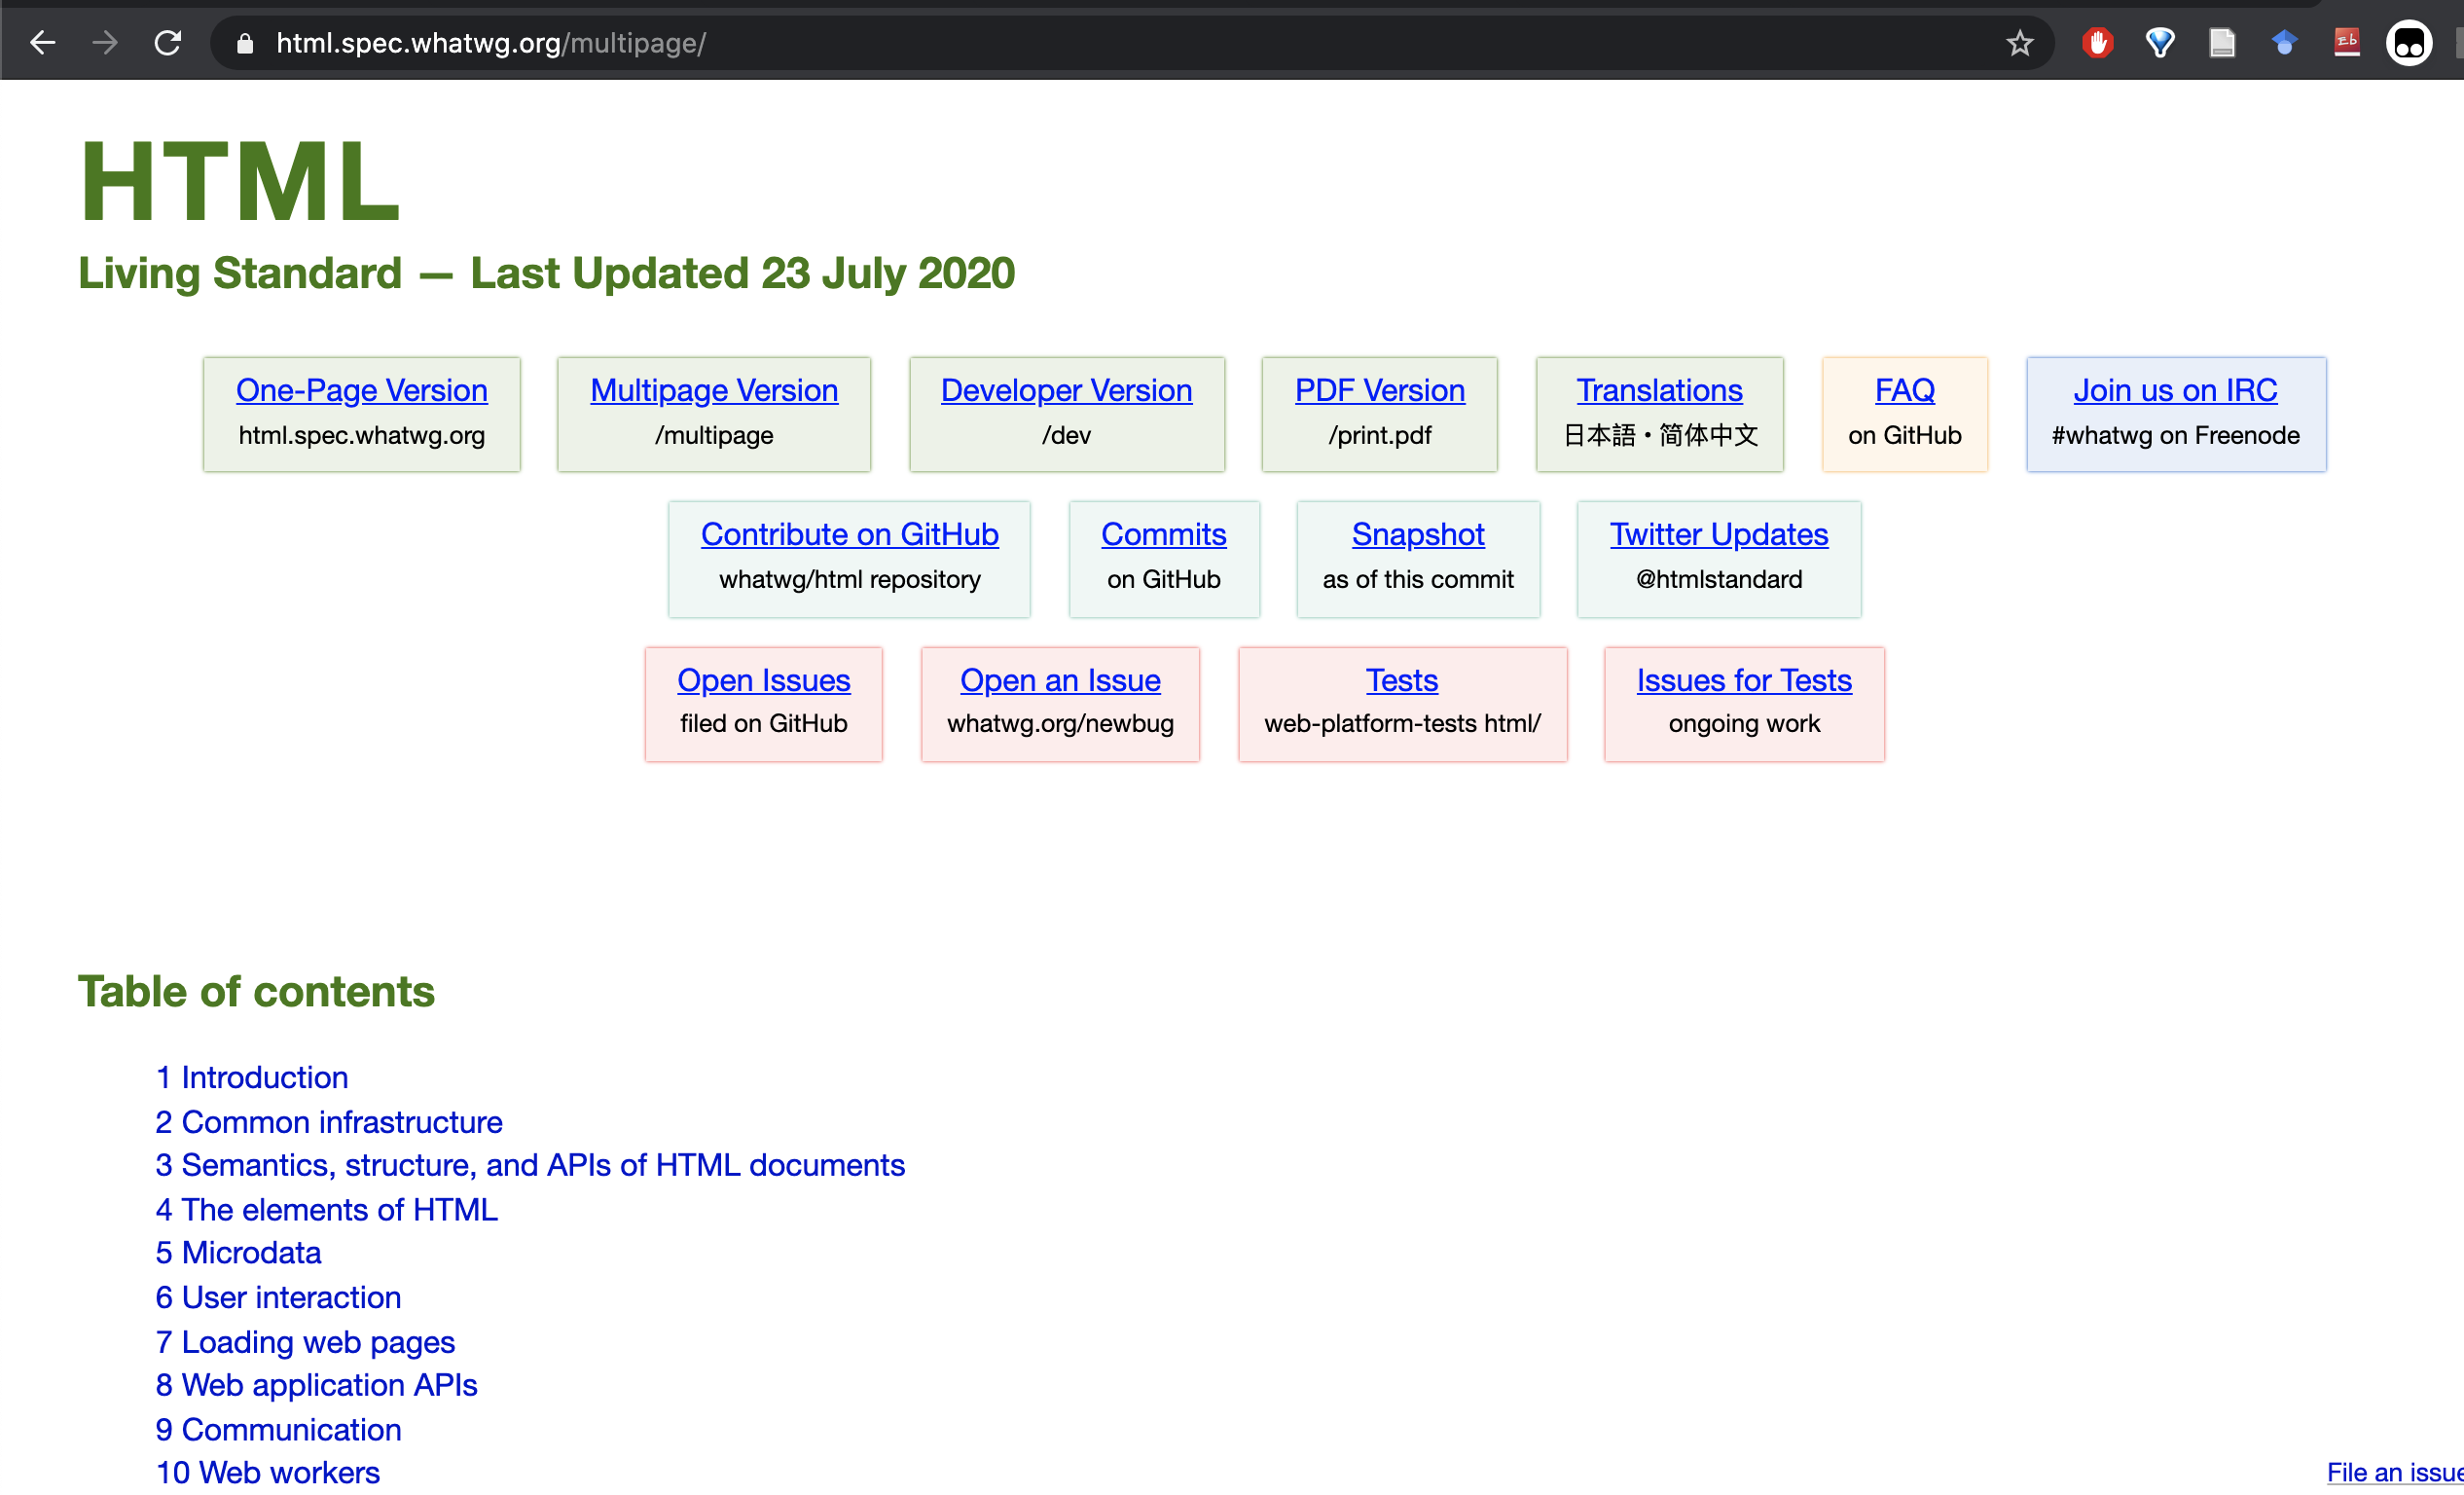
\includegraphics[trim=0cm 1cm 0cm 0cm, clip=true, width=0.75\textwidth]{img/html5standar}
\caption{HTML5 estandarra bizirik dago eta eguneraketak jasotzen jarraitzen du WHATWG webgunean: \href{https://html.spec.whatwg.org/multipage/}{https://html.spec.whatwg.org/multipage/}.}
\label{fig:quirksmode}
\end{figure}


\section{Historia apur bat}
\begin{alertinfo}{Hautazkoa}
Atal batzuk nahiko teknikoak bilaka daitezke. Hau bezalako ``Hautazko'' ohartxoak jarri ditugu horrelako azpiataletan, abisu gisa edo :)
\end{alertinfo}

HTML lengoaia hainbat bertsiotatik igaro da. Tim Berners Leek 1991n proposatu zuen HTMLren lehenengo zirriborroa, 18 etiketaz osatutakoa. Horietatik, 11 etiketa oraindik ere aurki daitezke HTML5en. Zirriborro horretan, \index{IETF} IETF (Internet Engineering Task Force) erakundeak 1993ko erdialdean HTML zehaztapenak argitaratu zituen. Ondoren, IETFk HTML espezifikazioa hobetzeko eta kudeatzeko 
``HTML Working Group'' izeneko taldea antolatu zuen. Talde horren lanaren lehenengo emaitza —beste enpresa eta erakunde batzuen ekarpena jaso ondoren, adibidez, Mosaic nabigatzaile aitzindariaren IMG etiketa— 1995ean plazaratu zen, HTML2 estandarra.

IETFk 1995ean HTML3ren proposamena jaso zuen, baina proposamena 6 hilabete geroago iraungi egin zen, inolako hobekuntzarik gabe. Bitartean, World Wide Web Consortium \index{W3C} (W3C) erakundea nabigatzaile propio bat garatzen hasia zen, \texttt{Arena} izenekoa, HTML3k proposatzen zituen berrikuntzak probatzeko asmoz (baita CSS estilo-orriak probatzeko ere). Garai hartan Netscape eta Internet Explorer sortu ziren, sekulako arrakastarekin. Nabigatzaileek eskatzen zituzten berrikuntzen kudeaketak eta HTMLk berak zuen ospeak IETFk zituen baliabideak gainezkatu zituzten. Hori dela eta, hurrengo urtetik hasita (1996), HTMLren espezifikazioa World Wide Web Consortium (W3C) erakundearen esku utzi zen.

W3C, IETFk egin zuen legez, kanpoko enpresen ekarpenak ere aztertu eta estandarra eguneratzen saiatu zen. Horren lehenengo fruitua 1997an izan zen, HTML4 estandarraren argitalpenarekin.

HTML 4.01 1999an argitaratu zen, nahiz eta akatsak zuzentzeko hainbat bertsio gehiago kaleratu behar izan zituzten 2001 arte.

2004an \index{WHATWG} WHATWG (\textit{Web Hypertext Application Technology Working Group}) lantaldea sortu zen, W3Ck HTMLren espezifikazioarekin zeraman erritmo motelari aurre egiteko. Baita W3C erakundeak HTML bertan behera utzi eta horren ordez XML lengoaian oinarritutako teknologiak sustatzeko hartutako erabakiari aurre egiteko ere.

WHATWG taldearen posta-zerrenda 2004ko ekainaren 4an sortu zen. Bertan Apple, Mozilla eta Opera nabigatzaileen ingeniariak HTML5 garatzen hasi ziren. WHATWGk Microsofteko ingeniari bati ere bertan parte hartzeko gonbita luzatu zion, baina ezezkoa jaso zuen.
 
2007an, WHATWGk bere HTML5en espezifikazioa W3Cren HTML garatzeko zuen lantaldeari eskaini zion, hortik abiatzeko haien lana. Izan ere, bertan adostu zuten HTML5 izena emango ziotela lantalde horien entregagaiari. Urte horretan bertan W3Ck eskaintza onartu zuen eta bi taldeen artean hainbat urtetan zehar lan egin ondoren, 2014ko urriaren 28an HTML5en lehenengo bertsio estandarra amaitu zuten.

% Zirriborro hau izan zen hain zuzen ere IETF (Internet Engineering Task Force) erakundeak 1993ko erdialdean erabili zuena HTML lengoaiaren lehenengo espezifikazioa argitaratzeko.

% \href{https://en.wikipedia.org/wiki/Mosaic_(web_browser)}{Mosaic (1993)}

% \href{https://en.wikipedia.org/wiki/Erwise}{Erwise (1992)}

% \href{https://en.wikipedia.org/wiki/ViolaWWW}{ViolaWWW (1992)}



\section{HTML5 etiketa berriak}

\subsection{HTML5 elementu berriak}

HTML5 bertsioak web dokumentuak eta aplikazioak sortzeko lengoaiaren bertsio zaharra hobetzen du, etiketa eta API (\textit{Application Programming Interfaces}) berriak eskainiz.

Zehazki, osagai grafiko berriak (\textit{<canvas>}, SVG —\textit{Scalable Vector Graphics}, grafiko bektorial-eskalagarriak—) eta multimedia (\textit{<audio>}, \textit{<video>}) eskaintzen ditu, \textit{plugin} edo API osagarririk erabili gabe.

Horretaz aparte, web dokumentuen edukiaren semantika hobetzeko elementuak gehitzen ditu: \textit{<section>}, \textit{<article>}, \textit{<header>} eta \textit{<nav>}, besteak beste.

HTML5en sorkuntzan hasiera-hasieratik dago errotuta gailu mugikorretarako web aplikazioak garatzeko lengoaia aproposa izan behar zuela, \textit{smartphone} eta \textit{tablet}-en ezaugarriak aprobetxatuz.

\subsection{Etiketa semantiko berriak}
Etiketa berriak edo HTML4 bertsioarekiko eguneratuak landuko ditugu hemen.

\index{DOCTYPE}\subsubsection{DOCTYPE hitzaurrea}
<!DOCTYPE html> hitzaurrearekin hasi behar dute HTML5en idatzitako web orriek. Horrekin, nabigatzaileak jakin ahalko du estandar berrienei jarraituz eraiki behar duela orria. DOCTYPE ingelesezko \textit{Document Type Declaration} (Dokumentu Motaren Erazagupena) hitzen akronimoa da.

Web orri baten HTML5 egitura zuzena dela egiaztatzeko online balidatzaileak erabil ditzakegu. Balidatzaile horiek egiten duten lehenengo gauza dokumentuaren sarrerari begiratzea da, jakin ahal izateko zer arauren kontra balioztatu behar duten uneko dokumentua. HTML5 lengoaian garatutako dokumentu zuzenek \textit{<!DOCTYPE html>} sarrerarekin hasi behar dute.

\vspace{0.5cm}
\begin{alertinfo}{Quirks mode}\index{Quirks mode}
    HTML5 diseinatzean ordura arte erabiltzen zen dokumentuen hitzaurrea erraztu nahi izan zen. Izan ere, nork gogoratzen du garai hartan erabiltzen zen hurrengo ``sarreratxoa''?
   \textit{<!DOCTYPE html PUBLIC \textquotedbl-//W3C/DTD HTML 4.01//EN\textquotedbl{}   \textquotedbl http://www.w3.org/TR/html4/strict.dtd\textquotedbl>}

Sarreratxo horri \texttt{DOCTYPE switch} deritzo. Agertuz gero, dokumentuak estandarrak betetzen dituela (estandarrei jarraituta idatzi dela) esan nahi du. Ez bada agertzen, estandarrei erdipurdi jarraituta edo estandarrak kontuan izan gabe idatzi dela esan nahi du (normalean webgune zaharretan gertatzen dena). Azken modu anarkiko horri \texttt{quirks mode} deritzo. HTML5en, DOCTYPE sarrera asko laburbildu da. Orain nahikoa da honela idaztea: \textit{<!DOCTYPE html>}
 
    \end{alertinfo}

\subsection{META etiketak}

META etiketak bilatzaileek erabiltzen dituzte batez ere jakin ahal izateko, automatikoki, zeintzuk diren dokumentuaren gako-hitzak (\textit{keywords}), hizkuntza, dokumentu mota edo erabilitako karaktere-jokoa. HTML5 sortu arte, hau zen maiz erabilitako META etiketa bat:
\begin{lstlisting}[numbers=none]
<meta http-equiv="content-type" content="text/html; charset=UTF-8">
\end{lstlisting}
Bertan, dokumentua HTMLz osatutako dokumentua zela zehazten zen. Baita UTF-8 karaktere-jokoa erabiltzen zela ere. Berriro, maiz erabilitako etiketa izateko, oso luzea, ezta? Orain, horrela laburbil daiteke, guztiz zuzena izanik:
\begin{lstlisting}[numbers=none]
<meta charset="utf-8">
\end{lstlisting}

Gauza bera gertatzen da estilo-orriak zehazteko garaian. Lehen honela idazten zena: 
\begin{lstlisting}[numbers=none]
<link type="text/css" rel="stylesheet" href="estiloak.css">
\end{lstlisting}
HTML5en beste era honetara idazten da:
\begin{lstlisting}[numbers=none]
<link rel="stylesheet" href="estiloak.css">
\end{lstlisting}
Edo JavaScript-en egindako \textit{skriptak} estekatzean lehen honela egiten zena: 
\begin{lstlisting}[numbers=none]
<script type="text/javascript" src="kodigoa.js"></script>
\end{lstlisting}
orain honela laburbildu da: 
\begin{lstlisting}[numbers=none]
<script src="kodigoa.js"></script>
\end{lstlisting}
Gauza bera orriaren hizkuntza adierazteko. Lehen:
\begin{lstlisting}[numbers=none]
<html xmlns="http://www.w3.org/1999/xhtml" lang="en" xml:lang="en"> 
\end{lstlisting}
orain:
\begin{lstlisting}[numbers=none]
<html lang="en">
\end{lstlisting}

Etiketa semantiko berriak \index{<header>}\index{<nav>}\index{<article>}\index{<section>}\index{<aside>}(\textit{<header>, <footer>, <nav>, <article>, <section>, <aside>}) hurrengo gaian jorratuko ditugu. Osagai grafiko berriak aztertzeko ere atal bereziak izango ditugu liburu honetan. Zehazki, \textit{<canvas>} eta <svg> etiketak 8. atalean zehazten dira eta multimediarekin lotutako etiketak, \textit{<audio>} eta \textit{<video>}, 9. atalean.

\section{Ariketak}

\begin{enumerate}

\item Bihurtu HTML5 formatura HTML4n programatutako lerro hauek:

\begin{lstlisting}[numbers=none]
<meta http-equiv="content-type"content="text/html; charset=UTF-8">
\end{lstlisting}
     
\begin{lstlisting}[numbers=none]
<link type="text/css" rel="stylesheet" href="estiloak.css">
\end{lstlisting}
    
\begin{lstlisting}[numbers=none]
<script type="text/javascript" src="kodigoa.js"></script>
\end{lstlisting}

\begin{lstlisting}[numbers=none]
<html xmlns="http://www.w3.org/1999/xhtml" lang="eu_ES" xml:lang="eu_ES">
\end{lstlisting}

\item Bihurtu HTML5 formatura HTML4n programatutako adibide hau:

\begin{lstlisting}[language=HTML,numbers=none]
<!DOCTYPE html PUBLIC "-//W3C//DTD XHTML 1.0 Strict//EN"
"http://www.w3.org/TR/xhtml1/DTD/xhtml1-strict.dtd">
<html xmlns="http://www.w3.org/1999/xhtml"
 lang="eu_ES"
 xml:lang="eu_ES">
 <head>
 <meta charset="utf-8" />
 <title>1. Ariketa </title>
 <link href="css/style.css" rel="stylesheet" />
 </head>
 <body>
 </body>
</html>
\end{lstlisting}
\end{enumerate}